%!TEX root = ../thesis.tex
%*******************************************************************************
%*********************************** First Chapter *****************************
%*******************************************************************************

\chapter{Introduction}  %Title of the First Chapter

\ifpdf
    \graphicspath{{Chapter1/Figs/Raster/}{Chapter1/Figs/PDF/}{Chapter1/Figs/}}
\else
    \graphicspath{{Chapter1/Figs/Vector/}{Chapter1/Figs/}}
\fi

\section{Preface}
During my PhD research, people asked me frequently about the problem I am working on. They were curious about materials physics is about, what it entails and what my research included. I always wonder those researchers who are able to give for outsiders a simple explanation about their work. They are able to describe their field as an interesting, high-end technology research field where their work is irreplaceable. But I was always suspicious whether their explanations were scientifically correct, and they really did what they said - or it was just something they would like to do.

My approach to explaining my field is two-fold. First I always try to demonstrate that what I am doing is nothing special and anybody with sufficient willpower could understand materials physics. The explanation has helped people to view me as a normal human being, who presents materials physics as a far more approachable field than to the stereotypical reputation of physics. So, when people ask me what I am doing, I reply the following:
\begin{quotation}
I do simple stuff. Some days I tinker strange springs and carry out measurements with a microscope. The other days I just push the buttons on my computer and write simple programs that simulate one of the defects in crystalline materials.
\end{quotation}
The next step is explaining why my work is useful and why it counts as science. I tell them that the special spring goes into a vacuum-chamber of a scanning electron microscope (SEM\nomenclature[z-SEM]{SEM}{scanning electron microscope}) in order to manipulate micron-sized crystals. I explain how some of the programs I have written can simulate the collective properties of the very important types of crystal defects, called dislocations, which determine the properties of the strange spring fabricated.

At the beginning of my thesis, let me ask the following question: why are dislocations special, why are they not just one of the crystal defects?

%********************************** %First Section  **************************************
\section{Importance of dislocations} %Section - 1.1 

``What vortex is in a fluid, that is a dislocation in a crystalline material. The major difference is that the number of dislocations is $10^{14}$ crossing a ${\rm{m}}^2$ area, so the average distance between dislocations is $10$~${\rm{nm}}$.''
The physical properties of crystalline materials are fundamentally influenced by the existence of lattice defects. Therefore, the mechanical properties of crystalline materials can be understood only on the basis of dislocation theory, because dislocations are the elementary units of plastic deformation. Thus, they play a major role in determining the technological properties of crystalline materials. Orován, Taylor and Polányi discovered dislocations in the 1930s and ever since a large amount of theoretical and experimental knowledge has been acquired in order to better understand the process of plastic deformation realised by dislocations.

Dislocations are one-dimensional crystal defects. Therefore their extension in the plane perpendicular to the line direction is in the order of the lattice spacing, while it is orders of magnitude larger in the third direction. It can vary from thousands of lattice spacing up to the size of the specimen.

In a early, naive picture of plastic deformation dislocations were excluded. According to a simplified mechanism, in case of an applied external stress, a part of the material is moved in the direction of the shear stress by a fraction of the lattice constant, with a parallel shear, and the boundary between the moved and untouched regions. The atom-atom bondings are distorted only along this boundary. By applying a large enough force, the system reaches an unstable equilibrium position, where all the atoms along the the boundary are moved by a half lattice constant. Then all the atoms in the upper half of the material, jump into a stable equilibrium position creating a new equilibrium configuration. This mechanism moves effectively the atoms on the one half of the imaginary boundary by a lattice constant.

In reality, however, another mechanism is responsible for plastic deformation. At the beginning, when an external force is applied, only the first couple of atoms are moved out of their equilibrium position near the crystal surface. By applying larger force they first go through an unstable equilibrium and then jump into a stable position leading to a shift of the defected region. This defect or disorder can easily move along the lattice leading to same result as the naive picture described above. This fundamentally different mechanism can be directly and indirectly verified both on a microscopic and a macroscopic scale.

Dislocations are not just one type of the crystal defects, but the most important one in the class of one-dimensional defects. Dislocations elucidate the differences between the crystal growth rates predicted by the classical theory and observed in experiments, which are significantly faster. They are also responsible for the discrepancy between the stress theoretically needed to induce plastic strain in perfect (i.e.\ defect-free) single crystals and the stress needed in real crystals (i.e.\ with dislocations) -- the latter is smaller by two orders of magnitude\footnote{Although dislocations describe why materials are softer than expected, one cannot suppose that dislocation density could be low enough to neglect dislocation-dislocation interactions. Such a presumption would lead to materials with softness never experienced. Therefore, the dislocation-dislocation interaction must be taken into account to predict the yield point in the right order of magnitude.}. In the section part a closer look on plastic deformation of a single crystal is presented to better demonstrate the importance of dislocations.

\subsection{Plastic deformation}

Consider Fig.~\ref{fig:plastic_deformation}, where a single crystal is subject to a tensile test. Since according to experimental evidences plastic deformation occurs in inclined planes, it is practical to resolve the applied tensile stress parallel and perpendicular of the plane selected by $XX'$. This is illustrated in Fig.~\ref{fig:plastic_deformation}b, where the force ${\mathbf{F}}$ is splitted into a ${{\mathbf{F}}_T}$ normal component (T for tensile) and into a ${{\mathbf{F}}_S}$ parallel component (S for shear). It is shown that a simple tensile force causes shear force leading to shear stress in a specimen.

Let us increase the tensile force until there is a permanent change in the shape (called plastic deformation) and then examine the surface under a microscope. A series of parallel lines can be seen on the surface, caused by small steps on the surface of the crystal. These are called slip lines or slip steps. By increasing the plastic strain, the height and the number of the slip lines increases. It seems that whole blocks of crystals have slipped one another in the direction of the resolved shear stress as shown in Fig.~\ref{fig:plastic_deformation}c. These slip lines are all parallel but not necessarily lie along the planes of maximum resolved shear. This indicates that not only the geometry but the crystallography of the crystal is what this process connected to. By taking a closer look on an atomistic scale (as shown in Fig.~\ref{fig:plastic_deformation}d) one can find that this is indeed the case: slip occurs only in preferred crystallographic planes (called slip planes) and in certain directions (called slip directions). The pair of the slip plane and its chosen slip direction called slip system. (A slip plane can allow multiple slip directions therefore more slip directions can be assigned to a slip plane.)

\begin{figure}[htbp!] 
\centering    
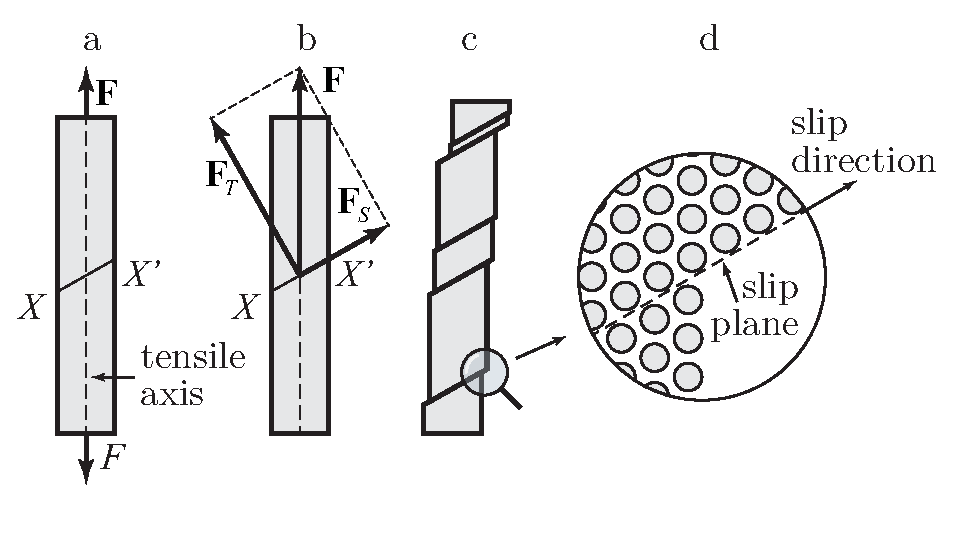
\includegraphics[width=0.6\textwidth]{slip_mechanism}
\caption[Plastic deformation]{The slip mechanism in plastic deformation.}
\label{fig:plastic_deformation}
\end{figure}

\subsection{The role of dislocations in modelling plasticity}
In engineering, plastic deformation is often described by phenomenological models in which constitutive relations are given between the stress, deformation, deformation rate and dislocation density\cite{Taylor1938307,HILL1972401,ASARO1985923,KUBIN1985397}. These models provide satisfactory results for a large variety of materials under general conditions for large enough samples. It turned out, however, that on a \si{\micro\meter} size scale the mechanical properties and the general behaviour of crystalline materials differ from what their phenomenological theories can predict \cite{FLECK1994475,mcelhaney_vlassak_nix_1998,Csikor251}. One example is the system size dependence of the plastic response observed experimentally, that is called size effect and it plays an important role in nanotechnology.

Due to the intense development in nanotechnology, it was inevitable to face the challenges of size effec to develop models correctly describing and modelling specimens in the \si{\micro\meter} size scale. The pressure from the side of the industry first led to the developement of new phenomenological, non-local models that describe the size effect successfully \cite{FLECK1994475,WalgraefAifantisJournal,WALGRAEF19851365}. However, they neglect the fact that plastic deformation are achieved by the motion of individual dislocations. They introduce gradient terms with coefficients containing length-dimensional parameters leading to a fundamental confrontation with the properties  of dislocations (see appendix \ref{sec:dimensionless_units}). These models are capable for capturing the hardening due to the smaller size of the specimen and they also explain some types of dislocation patterning, but due to their fundamental approach they are unable to account for some other phenomenon involving to involve the mechanism of dislocations. It has turned out that the plastic deformation of micropillars (micron-sized single crystal rods) is realised by intermittent, avalanche-like strain bursts in different regions of the sample as seen in Fig.~\ref{fig:avalanches_EM} \cite{DIMIDUK20054065,Dimiduk1188,Csikor251}. This behaviour makes the phenomenological models inefficient in predicting the plastic deformation on nanoscale.

\begin{figure}[htbp!] 
\centering    
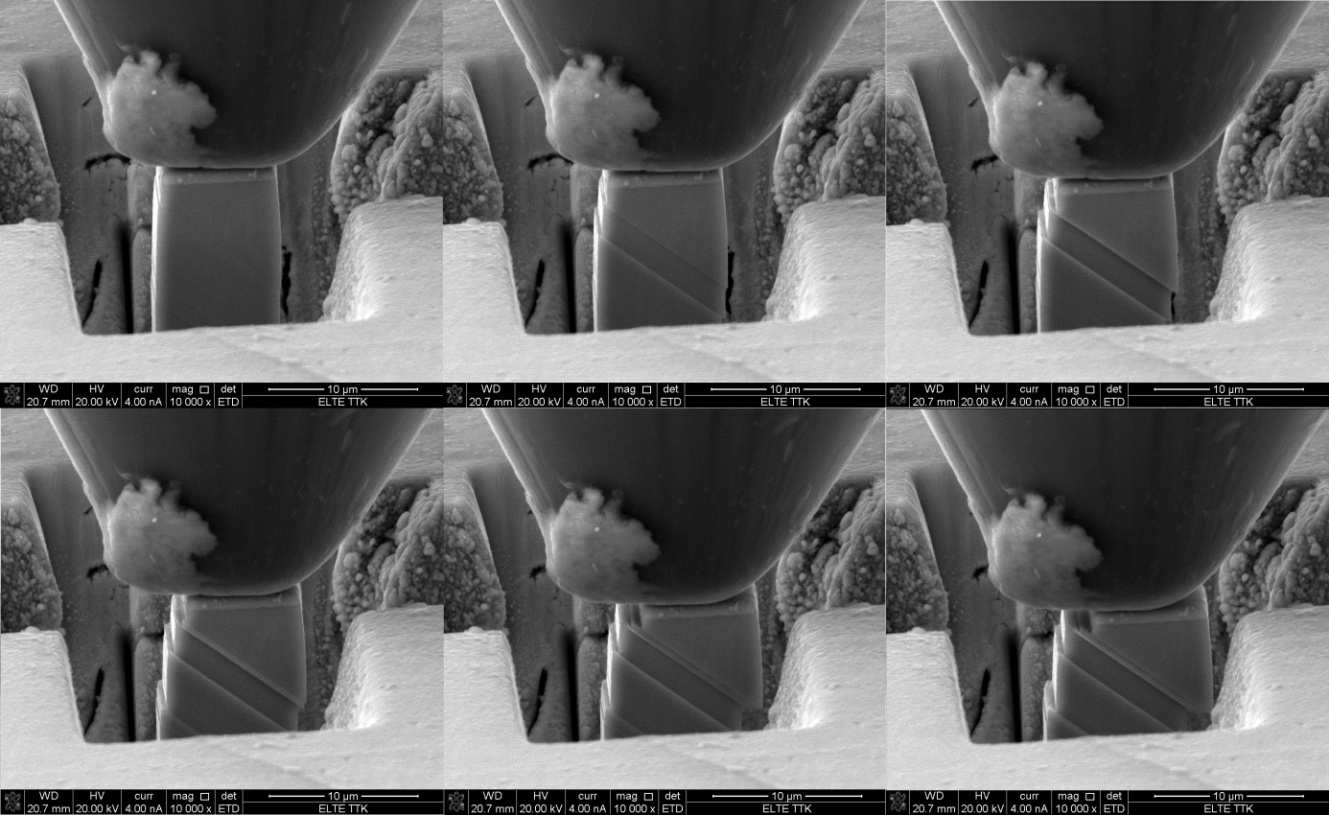
\includegraphics[width=0.8\textwidth]{bazalisZn28840.png}
\caption[Plastic deformation on nanoscale]{The slip mechanism in plastic deformation on nanoscale. The plastic response is not continuous, as it would be expected on macroscales. This picture has been taken at ELTE in a scanning electron microscope of a Zn single crystal oriented to basal slip system.}
\label{fig:avalanches_EM}
\end{figure}

\nomenclature[z-FIB]{FIB}{focused ion beam}      % first letter Z is for abbreviation
\nomenclature[z-CA]{CA}{cellular automaton}

%\nomenclature[a-F]{$F$}{complex function}                                                   %% first letter A is for Roman symbols

%\nomenclature[g-p]{$\pi$}{ $\simeq 3.14\ldots$}                                             %% first letter G is for Greek Symbols
%\nomenclature[g-i]{$\iota$}{unit imaginary number $\sqrt{-1}$}                      %% first letter G is for Greek Symbols
%\nomenclature[g-g]{$\gamma$}{a simply closed curve on a complex plane}  % %first letter G is for Greek Symbols
%\nomenclature[x-i]{$\oint_\gamma$}{integration around a curve $\gamma$} % %first letter X is for Other Symbols
%\nomenclature[r-j]{$j$}{superscript index}                                                       %% first letter R is for superscripts
%\nomenclature[s-0]{$0$}{subscript index}                                                        %% first letter S is for subscripts


%********************************** %Second Section  *************************************
\section{The actuality of the topic} %Section - 1.2

As described above, plastic strain is realised by and can be described with a fundamentally new mechanism in the regime of submicron scales. That is, the collective motion of dislocations causes a large intermittent strain burst -- called dislocation avalanches -- that in turn accumulates and creates plastic strain. This noisy behaviour can be handled only by statistical approaches.

The actuality of the topic is two-fold. First, state-of-the-art computers are able to run simulations on a much larger scale than ever before. Large supercomputers are capable to run molecular dynamic\footnote{See section \ref{sec:disloc_sim_md_sim}} simulations on \num{1000 x 1000 x 1000} atoms, displaying the core properties of dislocations in 3D. One cannot expect, however, that any of these computers can simulate a sample with size scale of \si{\micro\meter}. Simulations where the elementary units are the dislocations (or their segments) are also developed. They can capture the collective, avalanche-like behaviour of dislocations. Such models with further simplifications (e.g.\ 2D simulations) can be well handled on a larger computers that many universities and their departments have at their disposal.\footnote{These simplifications are still not sufficient in order to simulate a micron-sized sample. Consider a simulation with a mean dislocation density of \SI{e14}{\per m^2} in a micron-sized sample. In this case, one has to face \si{10^8} number of dislocations interacting with $10^8-1$ number of dislocations leading to a total of ${10^{16}}/2$ number of pair-interaction calculations per time steps. Supposing a lightning-fast CPU -- with a frequency of \SI{10}{\GHz}), and supposing that in each tick cycle the strongness of a pair-interaction force out of the $N^2/2$ can be calculated -- the time scale required to calculate all pair-interactions for just one single time step is in the order of months. Although this strong underestimation can be improved with parallel computing by involving hundred thousands of processors, the strong physical simplifications and huge technological challenges question the profitability of such trials.}

Second, state-of-the-art nanotechnology nowadays allows us to fabric and manipulate samples with a technology called FIB (focused ion beam) on the size scale of \si{\micro\meter}, on which the plastic deformation of the sample is deeply on the submicron scale. One can therefore recognise that nowadays the size scale one can simulate and fabric are in the same order of magnitude. This new key feature of the field has increased the possibility to verify models directly by physical, real specimen measurements and measurements can be suggested based on the results of computer simulations. Until now a large drawback of the technology was that the samples prepared with FIB in the vacuum chamber of the SEM were not deformed in the same device due to technical problems. Technological advancement also let us to develop a nanodeformation tool that can fit into the vacuum chamber of a SEM, facilitating to investigate in situ the emerging steps on the side of miropillars formed due to dislocation avalanches.

%********************************** % Third Section  *************************************
\section{The structure of the thesis}
In the next chapter, models describing crystal defects are presented with the focus on dislocation simulations, especially on continuum dislocation simulations. This is necessary in order to understand the models introduced in the latter parts.

The objective of this thesis is two-fold, just as the actuality of the topic. 
In the first half of the thesis, the topic is approached from a simulation point of view in chapter \ref{chapter:weakest_link}. A cellular automaton (CA) model is introduced to link model parameters between discrete dislocation dynamics \nomenclature[z-DDD]{DDD}{discrete dislocation dynamics}(DDD) and continuum dislocation dynamics (CDD) \nomenclature[z-CDD]{CDD}{continuum dislocation dynamics} models. The results are published in an article noted in chapter \ref{chapter:publications}, at point \hyperref[paper:A2]{[O1]}. A remarkable feature of the numerical model is that with further extensions of the CA model it is capable of describing materials which undergo strain softening, like metallic glasses. A striking property of the model, is that it is capable of describing single crystals just as metallic glasses. The details are described in the chapter \ref{chapter:disorder}, in which this feature is utilised to study fracture under strain softening in metallic glasses. The results are published in a paper, at point \hyperref[paper:A3]{[O2]} in chapter \ref{chapter:publications}. Finally, another CA model is introduced in chapter \ref{chapter:pattern} to study dislocation patterning. The results are presented along with a non-discretised model. The results have been also published in a paper, noted at point \hyperref[paper:A4]{[O3]} in chapter \ref{chapter:publications}.

In the second half, the topic of this thesis is approached from an experimental point of view, see chapter \ref{chapter:in_situ}. In order to investigate the properties of plastic deformation on a micron-scale, one has to produce a mass amount of samples and test them. The fabrication can be done by a FIB, a commercially available technology for electron microscopes. Another challenge is how to construct and calibrate a nanodeformation device (which fits into the vacuum chamber of a SEM) in order to conduct experiments. The device is coupled to an acoustic emission signal detector to exhibit the potential of the setup. The results achieved therewith has been already published in a paper, see point \hyperref[paper:A1]{[O4]} in chapter \ref{chapter:publications}.